% Fig. 1 design schematic (proposal). Standalone so it compiles to its own PDF for Science.
\documentclass[border=4pt]{standalone}
\usepackage[T1]{fontenc}
\usepackage{helvet}
\renewcommand{\familydefault}{\sfdefault}
\usepackage{tikz}
\usetikzlibrary{positioning, fit, calc, arrows.meta, backgrounds}

% Paper palette: GPT #0072B2, DeepSeek #D55E00, rule-based grey
\definecolor{gpt}{HTML}{0072B2}
\definecolor{ds}{HTML}{D55E00}
\definecolor{rule}{HTML}{6E6E6E}
\definecolor{coop}{HTML}{5A5A5A}
\definecolor{defect}{HTML}{E3E3E3}
\definecolor{act}{HTML}{8B1A1A}
\definecolor{panel}{HTML}{F6F6F6}

\begin{document}
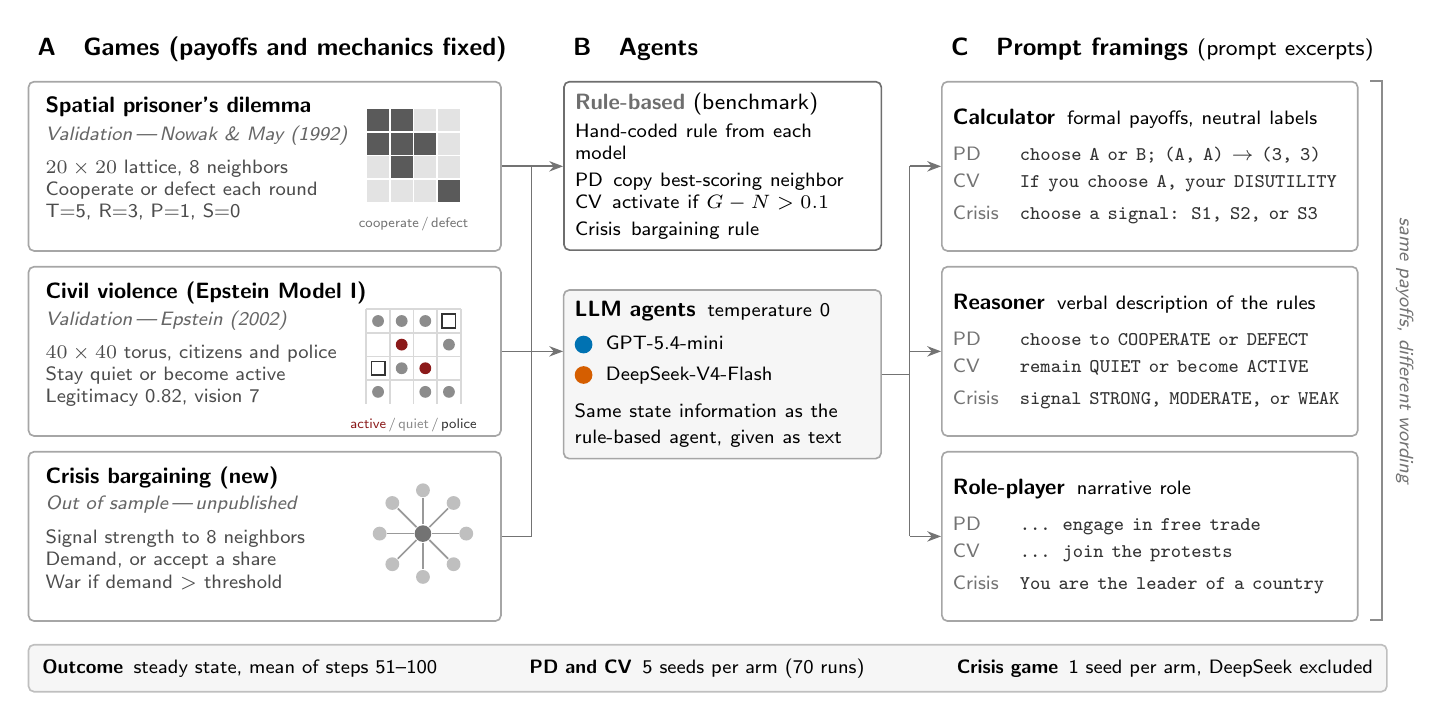
\begin{tikzpicture}[line width=0.6pt,
  font=\footnotesize,
  box/.style={draw=black!35, rounded corners=2pt, fill=white, inner sep=4pt, align=left, execute at begin node={\hyphenpenalty=10000\relax}},
  head/.style={font=\small\bfseries, anchor=west},
  tag/.style={font=\scriptsize\itshape, text=black!60, anchor=north west},
  arr/.style={-{Stealth[length=5pt]}, line width=0.6pt, black!55},
  snip/.style={font=\scriptsize\ttfamily, text=black!75, align=left, text width=4.6cm},
]

% =============== Panel A: games ===============
% Layout grid (cm): A x 0--6.0, B x 6.8--10.8, C x 11.6--17.0; boxes 2.15 tall, 0.2 gap (tops -0.4, -2.75, -5.1)
\newcommand{\gamebox}[5]{% #1 name, #2 top y, #3 title, #4 tag, #5 body
  \node[box, minimum width=6.0cm, minimum height=2.15cm, anchor=north west] (#1) at (0,#2) {};
  \node[anchor=north west, font=\footnotesize\bfseries] at ($(#1.north west)+(0.1,-0.08)$) {#3};
  \node[tag] at ($(#1.north west)+(0.1,-0.45)$) {#4};
  \node[anchor=north west, font=\scriptsize, align=left, text=black!70, text width=3.9cm] at ($(#1.north west)+(0.1,-0.88)$) {#5};
}
\node[head] at (0, 0) {A\quad Games (payoffs and mechanics fixed)};
\gamebox{pd}{-0.4}{Spatial prisoner's dilemma}{Validation\,|\,Nowak \& May (1992)}{$20\times20$ lattice, 8 neighbors\\Cooperate or defect each round\\T=5, R=3, P=1, S=0}
\gamebox{cv}{-2.75}{Civil violence (Epstein Model I)}{Validation\,|\,Epstein (2002)}{$40\times40$ torus, citizens and police\\Stay quiet or become active\\Legitimacy 0.82, vision 7}
\gamebox{ic}{-5.1}{Crisis bargaining (new)}{Out of sample\,|\,unpublished}{Signal strength to 8 neighbors\\Demand, or accept a share\\War if demand $>$ threshold}

% mini graphics, right side of each game box (x 4.3--5.75)
\begin{scope}[shift={(4.3,-0.75)}]
  \foreach \x/\y/\c in {0/0/coop,1/0/coop,2/0/defect,3/0/defect,
                        0/1/coop,1/1/coop,2/1/coop,3/1/defect,
                        0/2/defect,1/2/coop,2/2/defect,3/2/defect,
                        0/3/defect,1/3/defect,2/3/defect,3/3/coop}
    \fill[\c, draw=white, line width=0.6pt] (0.30*\x, -0.30*\y) rectangle ++(0.30,-0.30);
\end{scope}
\begin{scope}[shift={(4.3,-3.3)}]
  \draw[black!15] (0,0) grid[step=0.30] (1.2,-1.2);
  \foreach \x/\y in {0/0,2/0,3/1,1/2,0/3,2/3,3/3,1/0} \fill[black!45] (0.30*\x+0.15,-0.30*\y-0.15) circle (0.075);
  \foreach \x/\y in {1/1,2/2} \fill[act] (0.30*\x+0.15,-0.30*\y-0.15) circle (0.075);
  \foreach \x/\y in {3/0,0/2} \draw[black!80, line width=0.6pt] (0.30*\x+0.065,-0.30*\y-0.065) rectangle ++(0.17,-0.17);
\end{scope}
\begin{scope}[shift={(5.02,-6.15)}]
  \node[circle, fill=black!55, minimum size=6pt, inner sep=0] (c0) at (0,0) {};
  \foreach \a in {0,45,...,315} {
    \node[circle, fill=black!25, minimum size=5pt, inner sep=0] (n\a) at (\a:0.55) {};
    \draw[black!40, line width=0.6pt] (c0) -- (n\a);
  }
\end{scope}
\node[font=\tiny, text=black!55, anchor=north] at (4.9,-2.0) {cooperate\,/\,defect};
\node[font=\tiny, text=black!55, anchor=north] at (4.9,-4.55) {\textcolor{act}{active}\,/\,\textcolor{black!45}{quiet}\,/\,\textcolor{black!80}{police}};

% =============== Panel B: agents ===============
\node[head] at (6.8, 0) {B\quad Agents};
\node[box, draw=rule, line width=0.6pt, text width=3.75cm, anchor=north west] (rb) at (6.8, -0.4)
  {\textbf{\textcolor{rule}{Rule-based}} (benchmark)\\[2pt]
   \scriptsize Hand-coded rule from each model\\[2pt]
   \scriptsize PD\enspace copy best-scoring neighbor\\
   \scriptsize CV\enspace activate if $G-N>0.1$\\
   \scriptsize Crisis\enspace bargaining rule};
\node[box, fill=panel, text width=3.75cm, anchor=north west] (llm) at (6.8, -3.05)
  {\textbf{LLM agents}\enspace\scriptsize temperature 0\\[4pt]
   \tikz[baseline=-0.6ex]\fill[gpt] (0,0) circle (3.2pt);\; GPT-5.4-mini\\[3pt]
   \tikz[baseline=-0.6ex]\fill[ds] (0,0) circle (3.2pt);\; DeepSeek-V4-Flash\\[4pt]
   \scriptsize Same state information as the rule-based agent, given as text};

% games -> agents (spine at x = 6.4)
\foreach \g in {pd,cv,ic} \draw[black!55, line width=0.6pt] (\g.east) -- (6.4, 0 |- \g.east);
\draw[black!55, line width=0.6pt] (6.4, 0 |- pd.east) -- (6.4, 0 |- ic.east);
\draw[arr] (6.4, 0 |- pd.east) -- (6.8, 0 |- pd.east);
\draw[arr] (6.4, 0 |- cv.east) -- (6.8, 0 |- cv.east);

% =============== Panel C: framings ===============
\node[head] at (11.6, 0) {C\quad Prompt framings \normalfont\footnotesize(prompt excerpts)};
% one excerpt per game, each a single line (<= 32 characters of prompt text)
\newcommand{\pl}[2]{\makebox[0.85cm][l]{\textsf{\color{black!55}#1}}{\ttfamily\color{black!80}#2}}
\newcommand{\fbx}[7]{% #1 name, #2 top y, #3 title, #4 gloss, #5 PD, #6 CV, #7 Crisis
  \node[box, text width=5.0cm, minimum height=2.15cm, anchor=north west, align=left] (#1) at (11.6,#2)
    {\textbf{#3}\enspace\scriptsize #4\\[5pt]
     \scriptsize\pl{PD}{#5}\\[2pt]\pl{CV}{#6}\\[2pt]\pl{Crisis}{#7}};
}
\fbx{calc}{-0.4}{Calculator}{formal payoffs, neutral labels}
  {choose A or B; (A, A) $\rightarrow$ (3, 3)}{If you choose A, your DISUTILITY}{choose a signal: S1, S2, or S3}
\fbx{reas}{-2.75}{Reasoner}{verbal description of the rules}
  {choose to COOPERATE or DEFECT}{remain QUIET or become ACTIVE}{signal STRONG, MODERATE, or WEAK}
\fbx{role}{-5.1}{Role-player}{narrative role}
  {\ldots{} engage in free trade}{\ldots{} join the protests}{You are the leader of a country}

% llm -> framings (spine at x = 11.2)
\draw[black!55, line width=0.6pt] (llm.east) -- (11.2, 0 |- llm.east);
\draw[black!55, line width=0.6pt] (11.2, 0 |- calc.west) -- (11.2, 0 |- role.west);
\foreach \f in {calc,reas,role} \draw[arr] (11.2, 0 |- \f.west) -- (\f.west);

% bracket: same payoffs across framings
\draw[black!45, line width=0.6pt] (17.05,-0.4) -- (17.2,-0.4) -- (17.2,-7.25) -- (17.05,-7.25);
\node[rotate=-90, font=\scriptsize\itshape, text=black!55, anchor=south] at (17.25,-3.825) {same payoffs, different wording};

% =============== Bottom strip: measurement ===============
\node[draw=black!25, fill=panel, rounded corners=2pt, anchor=north west, inner sep=5pt, text width=16.9cm, align=left, font=\scriptsize] at (0,-7.55)
  {\hyphenpenalty=10000\textbf{Outcome}\enspace steady state, mean of steps 51--100\hfill
   \textbf{PD and CV}\enspace 5 seeds per arm (70 runs)\hfill
   \textbf{Crisis game}\enspace 1 seed per arm, DeepSeek excluded};

\end{tikzpicture}
\end{document}
